\section{Problem reductions}
Before presenting our formulation, some more direct reduction should be presented, not only to decrease the problem, but because they are also necessary for our new formulation to be correct.

\begin{myred}
    For a Target Set Selection instance $\mathcal{I} = \{G = (V,E), f\}$, and any $v \in V$ where $f(v) > \mathcal{N}_{G}(v)$, delete $v$, decrease the neighbors' threshold by one, and already add $v$ to the set of vertices that have to be initially infected.
\end{myred}

This reduction puts vertices that have to be in the minimum target set to infect the whole graph. In the following subsections, we will assume that the instances we are working with have all vertices with $\text{deg}(v) \geq f(v), \text{for} v \in V$, being necessary to prove properties we will use in the formulation.

\begin{figure}[!ht]
    %\newlength{\tempheight}
    %\setlength{\tempheight}{15ex}
    \centering
    \begin{subfigure}[t]{0.5\textwidth}
        \centering
         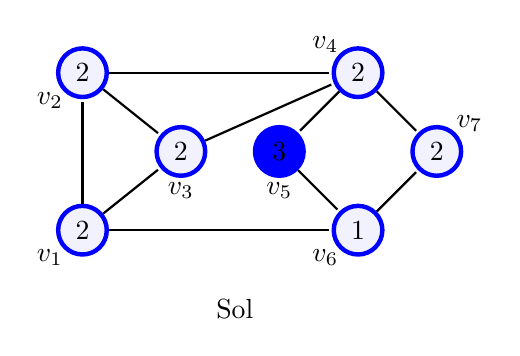
\begin{tikzpicture}[shorten >=1pt, auto, node distance=3cm, ultra thick]
    \tikzstyle{node_style} = [circle,draw=blue,fill=blue!5!]
    \tikzstyle{node_infected} = [circle,draw=blue,fill=blue!100!]
    \tikzstyle{edge_style} = [draw=black, line width=2, thick]
    \node[node_style] (v1) at (-2,-1) {2};
    \node[node_style] (v2) at (-2,1) {2};
    \node[node_style] (v3) at (-0.75,0) {2};
    \node[node_style] (v4) at (1.5,1) {2};
    \node[node_infected] (v5) at (0.5,0) {3};
    \node[node_style] (v6) at (1.5,-1) {1};
    \node[node_style] (v7) at (2.5,0) {2};
    
    \node[text width=2cm] at (0.7,-2) {Sol };
    \node [below left=3] at (v2) {$v_2$};
    \node [below left=3] at (v1) {$v_1$};
    \node [below=7] at (v3) {$v_3$};
    \node [above left=3] at (v4) {$v_4$};
    \node [below=7] at (v5) {$v_5$};
    \node [below left=3] at (v6) {$v_6$};
    \node [above right=3] at (v7) {$v_7$};

    
    \draw[edge_style]  (v1) edge (v2);
    \draw[edge_style]  (v1) edge (v3);
    \draw[edge_style]  (v2) edge (v3);
    \draw[edge_style]  (v1) edge (v6);
    \draw[edge_style]  (v2) edge (v4);
    \draw[edge_style]  (v3) edge (v4);
    \draw[edge_style]  (v4) edge (v5);
    \draw[edge_style]  (v5) edge (v6);
    \draw[edge_style]  (v4) edge (v7);
    \draw[edge_style]  (v6) edge (v7);
    \end{tikzpicture}
        \caption{Graph where the threshold value is inside each vertex. Notice that $\text{deg}(v_5) < f(v_5)$. We can use Reduction 1 in this Target Set Selection instance.}
        \label{fig:411}
    \end{subfigure}
    \begin{subfigure}[t]{0.5\textwidth}
        \centering
        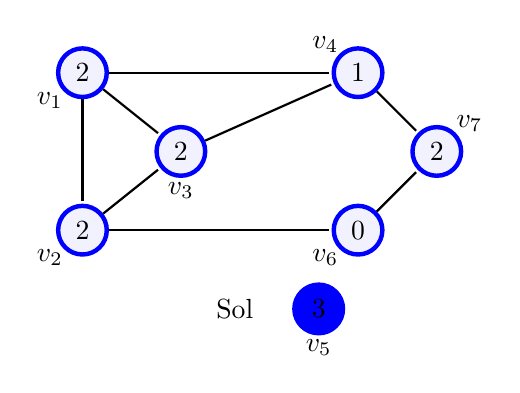
\begin{tikzpicture}[shorten >=1pt, auto, node distance=3cm, ultra thick]
    \tikzstyle{node_style} = [circle,draw=blue,fill=blue!5!]
    \tikzstyle{node_infected} = [circle,draw=blue,fill=blue!100!]
    \tikzstyle{edge_style} = [draw=black, line width=2, thick]
    \node[node_style] (v1) at (-2,1) {2};
    \node[node_style] (v2) at (-2,-1) {2};
    \node[node_style] (v3) at (-0.75,0) {2};
    \node[node_style] (v4) at (1.5,1) {1};
    \node[node_infected] (v5) at (1,-2) {3};
    \node[node_style] (v6) at (1.5,-1) {0};
    \node[node_style] (v7) at (2.5,0) {2};
    
    \node[text width=2cm] at (0.7,-2) {Sol };
    \node [below left=3] at (v2) {$v_2$};
    \node [below left=3] at (v1) {$v_1$};
    \node [below=7] at (v3) {$v_3$};
    \node [above left=3] at (v4) {$v_4$};
    \node [below=7] at (v5) {$v_5$};
    \node [below left=3] at (v6) {$v_6$};
    \node [above right=3] at (v7) {$v_7$};
    
    \draw[edge_style]  (v1) edge (v2);
    \draw[edge_style]  (v1) edge (v3);
    \draw[edge_style]  (v2) edge (v3);
    \draw[edge_style]  (v2) edge (v6);
    \draw[edge_style]  (v1) edge (v4);
    \draw[edge_style]  (v3) edge (v4);
    \draw[edge_style]  (v4) edge (v7);
    \draw[edge_style]  (v6) edge (v7);
    \end{tikzpicture}
        \caption{Instance resulting after applying Reduction 1 in the instance of Figure \ref{fig:411}}
        \label{fig:412}
    \end{subfigure}
\end{figure}

\begin{myred}
    For a Target Set Selection instance $\mathcal{I} = \{G = (V,E), f\}$,  and any $v \in V$ where $f(v) = 0$, delete $v$ and decrease thresholds. $v$ will not be in the solution.
\end{myred}
Also, we will need that for the whole graph, $f(v) > 0, v \in V$ as well.

\begin{figure}[!ht]
    %\setlength{\tempheight}{15ex}
    \centering%
    \begin{subfigure}[t]{0.5\textwidth}
        \centering%
         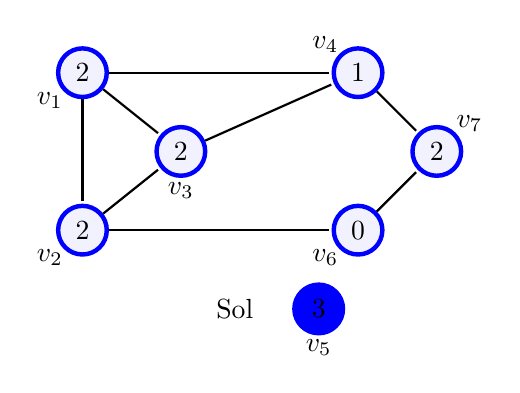
\begin{tikzpicture}[shorten >=1pt, auto, node distance=3cm, ultra thick]
    \tikzstyle{node_style} = [circle,draw=blue,fill=blue!5!]
    \tikzstyle{node_infected} = [circle,draw=blue,fill=blue!100!]
    \tikzstyle{edge_style} = [draw=black, line width=2, thick]
    \node[node_style] (v1) at (-2,1) {2};
    \node[node_style] (v2) at (-2,-1) {2};
    \node[node_style] (v3) at (-0.75,0) {2};
    \node[node_style] (v4) at (1.5,1) {1};
    \node[node_infected] (v5) at (1,-2) {3};
    \node[node_style] (v6) at (1.5,-1) {0};
    \node[node_style] (v7) at (2.5,0) {2};
    
    \node[text width=2cm] at (0.7,-2) {Sol };
    \node [below left=3] at (v2) {$v_2$};
    \node [below left=3] at (v1) {$v_1$};
    \node [below=7] at (v3) {$v_3$};
    \node [above left=3] at (v4) {$v_4$};
    \node [below=7] at (v5) {$v_5$};
    \node [below left=3] at (v6) {$v_6$};
    \node [above right=3] at (v7) {$v_7$};
    \draw[edge_style]  (v1) edge (v2);
    \draw[edge_style]  (v1) edge (v3);
    \draw[edge_style]  (v2) edge (v3);
    \draw[edge_style]  (v2) edge (v6);
    \draw[edge_style]  (v1) edge (v4);
    \draw[edge_style]  (v3) edge (v4);
    \draw[edge_style]  (v4) edge (v7);
    \draw[edge_style]  (v6) edge (v7);
    \end{tikzpicture}
        \caption{Graph where the threshold value is inside each vertex. Notice that $f(v_6) = 0$. We can use Reduction 2 in this Target Set Selection instance.}
        \label{fig:413}
    \end{subfigure}
    \begin{subfigure}[t]{0.5\textwidth}
        \centering
        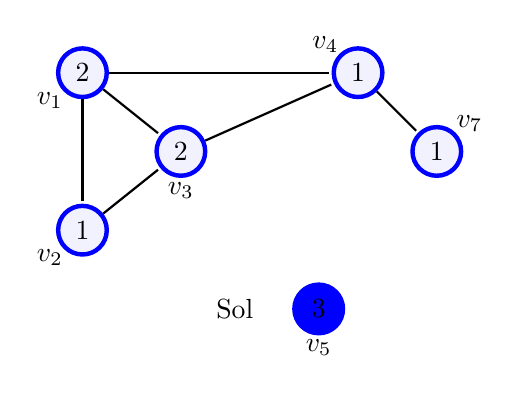
\begin{tikzpicture}[shorten >=1pt, auto, node distance=3cm, ultra thick]
    \tikzstyle{node_style} = [circle,draw=blue,fill=blue!5!]
    \tikzstyle{node_infected} = [circle,draw=blue,fill=blue!100!]
    \tikzstyle{edge_style} = [draw=black, line width=2, thick]
    \node[node_style] (v1) at (-2,1) {2};
    \node[node_style] (v2) at (-2,-1) {1};
    \node[node_style] (v3) at (-0.75,0) {2};
    \node[node_style] (v4) at (1.5,1) {1};
    \node[node_infected] (v5) at (1,-2) {3};
    \node[node_style] (v7) at (2.5,0) {1};
    
    \node[text width=2cm] at (0.7,-2) {Sol };
    \node [below left=3] at (v2) {$v_2$};
    \node [below left=3] at (v1) {$v_1$};
    \node [below=7] at (v3) {$v_3$};
    \node [above left=3] at (v4) {$v_4$};
    \node [below=7] at (v5) {$v_5$};
    \node [above right=3] at (v7) {$v_7$};
    
    \draw[edge_style]  (v1) edge (v2);
    \draw[edge_style]  (v1) edge (v3);
    \draw[edge_style]  (v2) edge (v3);
    \draw[edge_style]  (v1) edge (v4);
    \draw[edge_style]  (v3) edge (v4);
    \draw[edge_style]  (v4) edge (v7);
    \end{tikzpicture}
        \caption{Instance resulting after applying Reduction 2 in the instance of Figure \ref{fig:413}}
        \label{fig:414}
    \end{subfigure}
\end{figure}

\begin{myred}
    For a Target Set Selection instance $(G, f, Sol)$, reduced by Rule 1, and let  $v \in V (G)$ with $f(v) = \mathcal{N}_{G}(v) = 1$. Then, delete $v$ from $G$.
    \end{myred}
    An example for this reduction can be seen in Figure \ref{fig:415} and \ref{fig:416}.
Reduction 3 though will only help compressing our instances, being helpful in order to reduce the size of our problems, but not necessary in the next section proofs.


We can see an instance example in Figures \ref{fig:411} and the this instance reduced by Reduction 1 in \ref{fig:412}. Figures 
\ref{fig:413} and \ref{fig:414} show Reduction 2 and Figures \ref{fig:415} and \ref{fig:416} feature Reduction 3.

\begin{figure}[!ht]
    %\setlength{\tempheight}{15ex}
    \centering
    \begin{subfigure}[t]{0.4\textwidth}
        \centering
         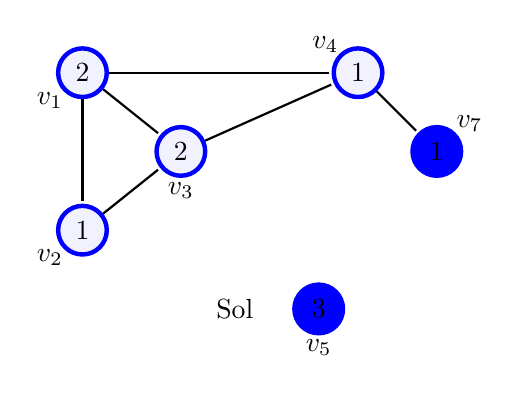
\begin{tikzpicture}[shorten >=1pt, auto, node distance=3cm, ultra thick]
    \tikzstyle{node_style} = [circle,draw=blue,fill=blue!5!]
    \tikzstyle{node_infected} = [circle,draw=blue,fill=blue!100!]
    \tikzstyle{edge_style} = [draw=black, line width=2, thick]
    \node[node_style] (v1) at (-2,1) {2};
    \node[node_style] (v2) at (-2,-1) {1};
    \node[node_style] (v3) at (-0.75,0) {2};
    \node[node_style] (v4) at (1.5,1) {1};
    \node[node_infected] (v5) at (1,-2) {3};
    \node[node_infected] (v7) at (2.5,0) {1};
    
    \node[text width=2cm] at (0.7,-2) {Sol };
    \node [below left=3] at (v2) {$v_2$};
    \node [below left=3] at (v1) {$v_1$};
    \node [below=7] at (v3) {$v_3$};
    \node [above left=3] at (v4) {$v_4$};
    \node [below=7] at (v5) {$v_5$};
    \node [above right=3] at (v7) {$v_7$};
    
    \draw[edge_style]  (v1) edge (v2);
    \draw[edge_style]  (v1) edge (v3);
    \draw[edge_style]  (v2) edge (v3);
    \draw[edge_style]  (v1) edge (v4);
    \draw[edge_style]  (v3) edge (v4);
    \draw[edge_style]  (v4) edge (v7);
    \end{tikzpicture}
         \caption{Graph where the threshold value is inside each vertex. Notice that $f(v_7) = \text{deg}(v_7) = 1$. We can use Reduction 3 in this Target Set Selection instance.}
        \label{fig:415}
    \end{subfigure}%
    \begin{subfigure}[t]{0.4\textwidth}
        \centering%
       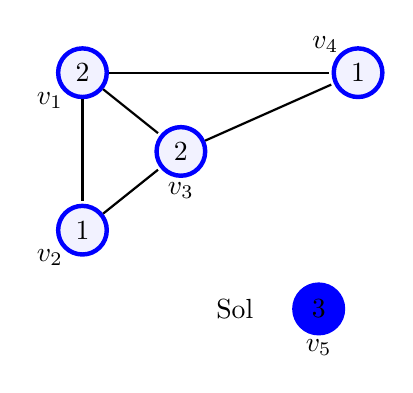
\begin{tikzpicture}[shorten >=1pt, auto, node distance=3cm, ultra thick]
    \tikzstyle{node_style} = [circle,draw=blue,fill=blue!5!]
    \tikzstyle{node_infected} = [circle,draw=blue,fill=blue!100!]
    \tikzstyle{edge_style} = [draw=black, line width=2, thick]
    \node[node_style] (v1) at (-2,1) {2};
    \node[node_style] (v2) at (-2,-1) {1};
    \node[node_style] (v3) at (-0.75,0) {2};
    \node[node_style] (v4) at (1.5,1) {1};
    \node[node_infected] (v5) at (1,-2) {3};
    
    
    \node[text width=2cm] at (0.7,-2) {Sol };
    \node [below left=3] at (v2) {$v_2$};
    \node [below left=3] at (v1) {$v_1$};
    \node [below=7] at (v3) {$v_3$};
    \node [above left=3] at (v4) {$v_4$};
    \node [below=7] at (v5) {$v_5$};
    
    \draw[edge_style]  (v1) edge (v2);
    \draw[edge_style]  (v1) edge (v3);
    \draw[edge_style]  (v2) edge (v3);
    \draw[edge_style]  (v1) edge (v4);
    \draw[edge_style]  (v3) edge (v4);
    \end{tikzpicture}
       \caption{Instance resulting after applying Reduction 3 in the instance of Figure \ref{fig:415}}
        \label{fig:416}
    \end{subfigure}
\end{figure}


\section{New formulation paradigm}

\subsection{General idea}

After analysing the previous introduced models, and defining some useful reductions in the previous sections, the idea was to get a model that would use some inherent property to the target set selection problem in order to improve its performance in more general graphs, since the previous models are said to perform better in sparse graph, more close to trees. With this in mind, we came up with a new paradigm to define this problem, based on the infection flow in a subset of vertices in the graph.

We will start by analysing one simple property that we know about the solution of a given instance of our problem.
\begin{myprop}
Given a Target Set Selection instance $ \mathcal{T} (G (V, E), f) $, where $G$ is our initial graph instance with set of vertices $V$ and edges $E$, and $f: V \to \mathbb{Z}^+$ our threshold function,  where Reductions 1 and 2 were applied. Then, a lower bound for the size of its Minimum Target Set is $\mathcal{C}$ is $\min_{v \ in V} f(v)$. 
\end{myprop},

\begin{proof}
This proof follows from the observation that, by contradiction, if you assume the number of initially infected vertices $|\mathcal{C}|$ are less then $ \min_{v \ in V} f(v) $,
since $f(v) \leq deg(v), \forall v \in V$, we know that $|\mathcal{C}| < \min_{v \ in V} f(v) \leq deg(v) < |V| $, we have that $\mathcal{C} \neq V$, so not all vertices are initially infected. Also, since $f(v) > 0, \forall v \in V$ no vertex will automatically infect itself. Now, we have that at least one vertex needs to be infected in order to spread the infection to the whole graph. So, we need $f(v) < |	\mathcal{C} \cap deg(v)|$ for some $v$. But $min_{v \in V} f(v) > |\mathcal{C}| \implies f(v) > |\mathcal{C}|, \forall v \in V \implies f(v) > |\mathcal{C} \cap deg(v)|$. Contradiction.
\end{proof}

With this property, we tried to generalize it for a subset of $V$. So, if $S \subset V$ was an isolated graph, we would know that for this set to be infected, at least $min_{v \in S}(f(v))$ vertices would have to infected at the beginning of the conversion process. When $S$ is not isolated from the rest of the graph, the difference are the edges between $S$ and $V \setminus S$ that can influence in the infection inside $S$. We know that these edges that go from $V \setminus S$ to $S$ can contribute to infect only the vertex they target with a "unit" of infection. We want to know at least how many vertices in $S$ would have to be infected at the beginning of the process in order to infect the whole subset. At least, all these edges will help infect $S$, and in this case each vertex would need to threshold function minus the number of edges coming from outside $S$,  $f(v) - |\mathcal{N}(v) \cap V \setminus S|$ to get infected, which means that $\min_{v \in V} |\mathcal{N}(v) \cap V \setminus S|$ is a lower bound for the vertices from $S$ that need to be in the target set solution. In the following section we prove this affirmation step by step.
 \begin{figure}[!ht]
    %\setlength{\tempheight}{15ex}
    \centering%
    \begin{subfigure}[t]{0.5\textwidth}
        \centering%
        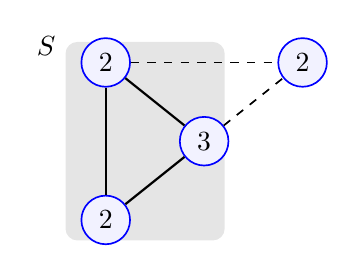
\begin{tikzpicture}[
    auto, % automatic node positioning
    node distance=2cm,
    semithick,
    bend angle=10,
    graybox/.style = {draw=gray!20, fill=gray!20, rounded corners},
    line/.style = {-&gt;, draw=black, thick},
    box/.style = {circle, draw=blue!50, fill=blue!20, minimum size=4mm}
    ]
    \tikzstyle{node_style} = [circle,draw=blue,fill=blue!5!]
    \tikzstyle{node_infected} = [circle,draw=blue,fill=blue!100!]
    \tikzstyle{node_infected2} = [circle,draw=blue,fill=blue!40!]
    \tikzstyle{edge_style} = [draw=black, line width=2, thick]
    \node (BBox) [graybox, minimum width=2cm, minimum height=2.5cm] at (-1.5cm, 0cm) {};
    \node [left] at (BBox.130) {$S$};
    \node[node_style] (v1) at (-2,1) {2};
    \node[node_style] (v2) at (-2,-1) {2};
    \node[node_style] (v3) at (-0.75,0) {3};
    \node[node_style] (v4) at (0.5,1) {2};
    
    \draw[edge_style]  (v1) edge (v2);
    \draw[edge_style]  (v1) edge (v3);
    \draw[edge_style]  (v2) edge (v3);
    \draw[dashed] (v1) edge (v4);
    \draw[dashed]  (v3) edge (v4);
    \end{tikzpicture}
        \caption{Instance where the threshold of each vertex is inside the node. Notice that the edges are between $S$ and $V \setminus S$.}
    \label{fig:416a}
    \end{subfigure}%
    \begin{subfigure}[t]{0.5\textwidth}
        \centering%
        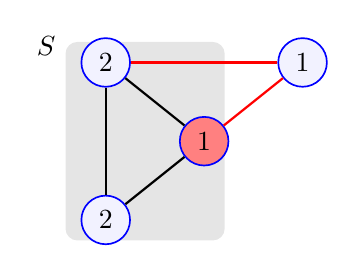
\begin{tikzpicture}[
    auto, % automatic node positioning
    node distance=2cm,
    semithick,
    bend angle=10,
    graybox/.style = {draw=gray!20, fill=gray!20, rounded corners},
    line/.style = {-&gt;, draw=black, thick},
    box/.style = {circle, draw=blue!50, fill=blue!20, minimum size=4mm}
    ]
    \tikzstyle{node_style} = [circle,draw=blue,fill=blue!5!]
    \tikzstyle{node_infected} = [circle,draw=blue,fill=red!50!]
    \tikzstyle{node_infected2} = [circle,draw=blue,fill=blue!40!]
    \tikzstyle{edge_style} = [draw=black, line width=2, thick]
    \tikzstyle{edge_dashed} = [draw=red, line width=4, thick]
    \node (BBox) [graybox, minimum width=2cm, minimum height=2.5cm] at (-1.5cm, 0cm) {};
    \node [left] at (BBox.130) {$S$};
    \node[node_style] (v1) at (-2,1) {2};
    \node[node_style] (v2) at (-2,-1) {2};
    \node[node_infected] (v3) at (-0.75,0) {1};
    \node[node_style] (v4) at (0.5,1) {1};
    
    \draw[edge_style]  (v1) edge (v2);
    \draw[edge_style]  (v1) edge (v3);
    \draw[edge_style]  (v2) edge (v3);
    \draw[edge_dashed] (v1) edge (v4);
    \draw[edge_dashed]  (v3) edge (v4);
    \end{tikzpicture}
        \caption{Thresholds were updated to their lower bound value $f(v) - | \mathcal{N}(v) \cap V \setminus S$. In this case, the lower bound for the target set size in $S$ is $min_{v \in S} f(v) - | \mathcal{N}(v) \cap V \setminus S = 1$.}
        \label{fig:416b}
    \end{subfigure}
\end{figure}
    %\centering{For $\mathcal{C}$ instance solution, $ |\mathcal{C} \cap S| \geq min_{v \in S} (f(v))$}

Based on this idea, we started to prove some properties regarding subsets $S$ of $V$.

\subsection{Graph Subset Properties}

Given an reduced instance $\mathcal{T}(G(V, E), f)$ as defined previously, in the Equation \ref{eq:2} we define the cut-set size as
  \begin{equation}\label{eq:2}
\delta(S) = |\{v_1v_2 \in E:  v_1 \in S , v_2 \in (V\setminus S)\} |
\end{equation}

Given a graph, a subset $S$, and minimum target set where the initial infected labels are given by $\mathcal{C}$, label that indicates if a vertex is infected $(1)$, or not $(0)$, we will be interested in sets $S$ where $\min_{v \in S} (f(v)) > \delta(S)$, so the following propositions can be proved.

\begin{myprop}
Given a set $S$ and $\mathcal{C}$,  %$\min_{v \in S} (f(v))$ and $\delta(S)$ as seen before, 
we have that
\begin{equation}
|\mathcal{C} \cap S | \geq \min_{v \in S} (f(v)) - \delta (S)
\end{equation}
\end{myprop}
%\footnote{não precisa nem $\min_{v \in S} (f(v))$ nem $\delta$ são operações já definidas }
\begin{proof} 
%This proof is simple.\footnote{tirar} 
First, we consider the case where every vertex in S is initially infected:
In this case, we know that $|\mathcal{C} \cap S | = |S|$. We also know that $f(v) \leq \mathcal{N}_G(v) $.  Besides, we notice that $\min_{v \in S} (f(v)) \leq f(v) \leq \mathcal{N}_G(v), v \in S$. So, if $ \delta(S)$ is the number of edges between $S$ and $V \setminus S$ . So, this implies that
\begin{equation}
\min_{v \in S} (f(v)) - \delta (S) \leq \mathcal{N}_G(v) \cap S  \leq |S| = |\mathcal{C} \cap S | 
\end{equation}
as we wanted to prove.

Now, suppose we have at least one vertex not infected at the beginning of the process. Let the first vertex of S %\footnote{of $S$}
to get infected after the process begins %\footnote{to get infected after the process begins} \footnote{como garante que esse vértice existe. Tem que excluir o caso em que todos os vértices de S estão infetados no começo} 
be $u$, where $u \notin C_0(S)$. We know that  $\min_{v \in S} (f(v)) \leq f(u)$ by definition of $\min_{v \in S} (f(v))$, and that $u$ can have, at most,  $\delta(S)$ infected neighbors outside $S$, so, to infect $u$, we need at least $f(u) -\delta(S)$. So, we know that, $|\mathcal{C} \cap S | \geq f(u) - \delta(S) \geq \min_{v \in S} (f(v)) - \delta(S) $.
\end{proof}

Let $\mathcal{N}_G(v)$ be the set of neighbors of a given vertex $v \in V(G)$.

\begin{myprop}
Given a set $S$,  $c_0$,  $\min_{v \in S} (f(v))$ and $\delta(S)$ as seen before, we have that 
\begin{equation}
|\mathcal{C} \cap S | \geq \min_{v \in S} (f(v)) - \max_{v \in S} (|\mathcal{N}_G(v) \cap (V \setminus S)|)
\end{equation}
\end{myprop}
\begin{proof}
As before, we consider two cases: 

First, we consider the case where every vertex in S is initially infected. We know that $|\mathcal{C} \cap S | = |S|$ and  $f(v) \leq \mathcal{N}_G(v) $.  Besides, we have that $\min_{v \in S} (f(v)) \leq f(v) \leq \mathcal{N}_G(v), v \in S$.  So, this implies that
\begin{gather}
\min_{v \in S} (f(v)) - \max_{v \in S} (|\mathcal{N}_G(v) \cap (V \setminus S)|) =\\
\min_{v \in S} (f(v))  - \max_{v \in S} (|\mathcal{N}_G(v) \cap (V \setminus S)|) \leq \\
f(v) - |\mathcal{N}_G(v) \cap (V \setminus S)| \leq \\ 
{N}_G(v)  - |\mathcal{N}_G(v) \cap (V \setminus S)| = \\ 
\mathcal{N}_G(v) \cap S  \leq\\  |S| = |\mathcal{C} \cap S | 
\end{gather}
as we wanted to prove.

Second, the case where at least one vertex was not infected in the beginning of the process. 
As before %\footnote{as before}%
, let $u \in S$ be the first vertex to be infected, where $u \notin C_0(S)$,    

$|{N}_G(u) \cap (V \setminus S)| \leq \max_{v \in S} (|\mathcal{N}_G(v) \cap (V \setminus S)|) \implies$ 

$\min_{v \in S} (f(v)) - |{N}_G(u) \cap (V \setminus S)| \geq \min_{v \in S} (f(v)) - \max_{v \in S} (|\mathcal{N}_G(v) \cap (V \setminus S)|) $.

Knowing that , by definition,  $f(u) \geq \min_{v \in S} (f(v))  \implies $ 

$f(u) - |{N}_G(u) \cap (V \setminus S)| \geq \min_{v \in S} (f(v)) - |{N}_G(u) \cap (V \setminus S)| \geq \min_{v \in S} (f(v)) - \max_{v \in S} (|\mathcal{N}_G(v) \cap (V \setminus S)|)  \implies$

$f(u) - |{N}_G(u) \cap (V \setminus S)|  \geq \min_{v \in S} (f(v)) - \max_{v \in S} (|\mathcal{N}_G(v) \cap (V \setminus S)|)  \implies$

%If $u$ was the first to be infected, we know that $|\mathcal{C} \cap S | \geq f(u) -  |{N}_G(u) \cap (V \setminus S)|$, since these are the only possibly infected neighbors of $u$\footnote{, 
Since $|{N}_G(u) \cap (V \setminus S)|$ is a maximum on the number of vertices outside $S$ that can help $u$ to become infected. Now, we have that:

$|\mathcal{C} \cap S | \geq f(u) - |{N}_G(u) \cap (V \setminus S)|  \geq \min_{v \in S} (f(v)) - \max_{v \in S} (|\mathcal{N}_G(v) \cap (V \setminus S)|)  \implies$

$|\mathcal{C} \cap S | \geq \min_{v \in S} (f(v)) - \max_{v \in S} (|\mathcal{N}_G(v) \cap (V \setminus S)|)$.

\end{proof}
\begin{mylemma}
Given a set $S$,  $|\mathcal{C} \cap S | $,  $\min_{v \in S} (f(v))$ and $\delta(S)$ as seen before, and we have that 
\begin{equation}
|\mathcal{C} \cap S | \geq  \min_{v \in S} (f(v) - |\mathcal{N}_G(v) \cap (V \setminus S)| ) 
\end{equation}
\end{mylemma}
\begin{proof}
If all vertices in $S$ were initially infected: Similar to the proof shown before,  for $v \in S$:
\begin{gather}
\min_{v \in S} (f(v) - |\mathcal{N}_G(v) \cap (V \setminus S)| ) \leq \\
f(v) - |\mathcal{N}_G(v) \cap (V \setminus S)| \leq \\ 
{N}_G(v)  - |\mathcal{N}_G(v) \cap (V \setminus S)| = \\ 
\mathcal{N}_G(v) \cap S  \leq |S| = \\
|\mathcal{C} \cap S | 
\end{gather}

proving this part of the proposition.
Now, for the case where at least one vertex was not initially infected.
We assume that  $|\mathcal{C} \cap S | <  \min_{v \in S} (f(v) - |\mathcal{N}_G(v) \cap (V \setminus S)|) $. We will prove that no $u \in S, u \notin C_0(S)$ can be infected.

Assume that $u \in S$ was the first vertex we attempted to infect, and $u \notin C_0(S)$. We want to proof that $|\mathcal{C} \cap S | + |\mathcal{N}_G(u) \cap (V \setminus S)| < f(u)$, no matter which $u$ is chosen, therefore we don't have a first vertex being infected.  
By hypothesis, we have:
\begin{center}
$|\mathcal{C} \cap S | <  \min_{v \in S} (f(v) - |\mathcal{N}_G(v) \cap (V \setminus S)|) \leq f(u) - |\mathcal{N}_G(u) \cap (V \setminus S)| \implies$

$|\mathcal{C} \cap S | <  f(u) - |\mathcal{N}_G(u) \cap (V \setminus S)| \implies$

$|\mathcal{C} \cap S | + |\mathcal{N}_G(u) \cap (V \setminus S)|<  f(u)$.
\end{center}
\end{proof}

\begin{mytheo} Given a Target Set Selection Instance $\mathcal{T}(G, f)$, $\mathcal{C} \subseteq V$ vertex set,   
\begin{equation}
\mathcal{C} \textit{ is convergent set in instance } \mathcal{T}(G, f) \iff |\mathcal{C} \cap S|\geq  \min_{v \in S} (f(v) - |\mathcal{N}_G(v) \cap (V \setminus S)| ) 
\end{equation}\end{mytheo} 
\begin{proof}
First, we proved the implication $\mathcal{C} \implies |\mathcal{C} \cap S| \geq  \min_{v \in S} (f(v) - |\mathcal{N}_G(v) \cap (V \setminus S)| )  $in the previous lemma. 

For the implication's other direction, assuming $\mathcal{C}$ is not convergent, we will prove that exists at least one $S$ where $|\mathcal{C} \cap S| <  \min_{v \in S} (f(v) - |\mathcal{N}_G(v) \cap (V \setminus S)| )  $. $\mathcal{C}$ is not convergent,  which means that if we simulate the spread of infection through the graph, not all vertices are infected. Take this set of infected vertices as $S$. 

Now we know that $ |\mathcal{C} \cap S| = 0 < \min_{v \in S} (f(v) - |\mathcal{N}_G(v) \cap (V \setminus S)| )$, otherwise, if for any $u \in S, f(u) - |\mathcal{N}_G(u) \cap (V \setminus S)| \leq 0 \implies f(u) \leq   |\mathcal{N}_G(u) \cap (V \setminus S)|$, which means $u$ would have been infected by the vertices outside $S$, contradiction.
\end{proof}


\subsection{Model and Constraints Found}

Based of the theorem previosly shown, we know, we know that if we find $\mathcal{C}$ convergent set, then any subset $S \subseteq V$ should hold for the inequality
\begin{equation}
    |\mathcal{C} \cap S| \geq \min_{v \in S} (f(v) - |\mathcal{N}_G(v) \cap (V \setminus S)| ) 
\end{equation}
We will be using this to define our model, where first we provide an empty $\mathcal{C}$. We will find an $S$ that violates equation , which means
\begin{equation}
    |\mathcal{C} \cap S| < \min_{v \in S} (f(v) - |\mathcal{N}_G(v) \cap (V \setminus S)| ) 
\end{equation}
When $\mathcal{C}$ is empty, if $S $
\begin{myprop}
For any $\mathcal{C}$ possible target set, if $|S| = 1$, than $S$ does not define a violated inequality.
\end{myprop}
\begin{proof}
Considering the premises guaranteed, we know that $\mathcal{N}_G(v) \geq f(v), v \in V$. With $S = \{v\}$, we have that

$\min_{v \in S} (f(v) - |\mathcal{N}_G(v) \cap (V \setminus S)| ) = f(v) - N_G(v)  < 0$ 

implying  that the inequality is never violated, since the following is always true:  

$|\mathcal{C} \cap S | \geq 0 \geq\min_{v \in S} (f(v) - |\mathcal{N}_G(v) \cap (V \setminus S)|) $ 
\end{proof}

\begin{myprop}
Given an $S$ that does not induce a connected graph, and $S$ generates a violated inequality, then exist an a $S' \subset S$, such that $S'$ induce a connected graph and $|\mathcal{C} \cap S | <  \min_{v \in S'} (f(v) - |\mathcal{N}_G(v) \cap (V \setminus S')|) $ will generate a violated inequality
\end{myprop}
\begin{proof}
Here, we first find the $v = \text{argmin}_{v \in S} (f(v) - |\mathcal{N}_G(v) \cap (V \setminus S)|)$. This $v$ is in a connected component in $S$, lets call it $S'$. It follows that $|\mathcal{C} \cap S' | \leq |\mathcal{C} \cap S | <  \min_{v \in S'} (f(v) - |\mathcal{N}_G(v) \cap (V \setminus S')|) $, proving $S'$ does also define a violated inequality. 
\end{proof}

\begin{myprop}
$ | N_G(v) \cap \mathcal{C}|  \geq f(v) \implies v \neq \text{argmin} (f(v) - |N_G(v) \cup V\setminus S|)$ , for $\forall S \subset V$
\end{myprop}
\begin{proof}
<Don't know what this proposition meant.>
\end{proof}

Write here algorithm that: starts infecting 1 vertex. Starts the process. If the process won't stop, create a violated inequality where S is the set of vertices that has not been infected. Do it till you infect all graph. This will generate a optimal solution for the problem here.
\begin{myprop}
This algorithm generates a model for the problem PCP
\end{myprop}
\begin{proof}

\end{proof}
Based on this results, create heuristic based on Prim's algorithm that creates S's based on a greedy choice 


After the results previously shown, that guarantee properties of any given $S$ set of vertices and $c_0$ solution to the target set selection problem, we can derive that, given a integer solution to the initial given model, if the properties proven above hold, then we have a viable solution, otherwise, if we find an S that does not hold that property, immediately we can derive a new constraint to our problem. We will name this constraint, our violated inequalities, that will be added to the model, and guarantee the model converges to the optimal solution.

%\section{Constraints}

%\section{Model}
